%! BibTeX Compiler = biber
%TC:ignore
\documentclass{article}

\usepackage{xcolor, colortbl}
\definecolor{BLUELINK}{HTML}{0645AD}
\definecolor{DARKBLUELINK}{HTML}{0B0080}
\PassOptionsToPackage{hyphens}{url}
\usepackage[colorlinks=false]{hyperref}
% for linking between references, figures, TOC, etc in the pdf document
\hypersetup{colorlinks,
    linkcolor=DARKBLUELINK,
    anchorcolor=DARKBLUELINK,
    citecolor=DARKBLUELINK,
    filecolor=DARKBLUELINK,
    menucolor=DARKBLUELINK,
    urlcolor=BLUELINK
} % Color citation links in purple
\PassOptionsToPackage{unicode}{hyperref}
\PassOptionsToPackage{naturalnames}{hyperref}

\usepackage{biorxiv}
\usepackage[backend=biber,eprint=false,isbn=false,url=false,intitle=true,style=nature,date=year]{biblatex}
\addbibresource{codon_models.bib}

\usepackage{url}
\usepackage{amssymb,amsfonts,amsmath,amsthm,mathtools}
\usepackage{lmodern}
\usepackage{xfrac, nicefrac}
\usepackage{bm}
\usepackage{listings, enumerate, enumitem}
\usepackage[export]{adjustbox}
\usepackage{graphicx}
\usepackage{bbold}
\usepackage{pdfpages}
\pdfinclusioncopyfonts=1
\usepackage{lineno}

\newcommand{\NS}[1]{\textcolor{red}{\textbf{\emph{[NS: #1]}}}}

\newcommand{\UniDimArray}[1]{\bm{#1}}
\newcommand{\BiDimArray}[1]{\bm{#1}}
\DeclareMathOperator{\E}{\mathbb{E}}
\DeclareMathOperator{\Var}{\textrm{Var}}
\newcommand{\der}{\textrm{d}}
\newcommand{\e}{\textrm{e}}
\newcommand{\avg}[1]{\left< #1 \right>} % for average
\newcommand{\Ne}{N_{\textrm{e}}}
\newcommand{\proba}{\mathbb{P}}
\newcommand{\pfix}{\proba_{\textrm{fix}}}
\newcommand{\dn}{d_N}
\newcommand{\ds}{d_S}
\newcommand{\dnds}{\dn / \ds}
\newcommand{\Sphy}{S_{0}}
\newcommand{\Sphyclass}{\mathcal{C}}
\newcommand{\SphyMean}{\overline{\Sphy}}
\newcommand{\divStrongDel}{\Sphy < -3}
\newcommand{\divDel}{-3 < \Sphy < -1}
\newcommand{\divWeakDel}{-1 < \Sphy < 0}
\newcommand{\divWeakAdv}{0 < \Sphy < 1}
\newcommand{\divAdv}{ \Sphy > 1}
\newcommand{\PdivStrongDel}{\proba \left[ \divStrongDel \right]}
\newcommand{\PdivDel}{\proba \left[ \divDel \right]}
\newcommand{\PdivWeakDel}{\proba \left[ \divWeakDel \right]}
\newcommand{\PdivWeakAdv}{\proba \left[ \divWeakAdv \right]}
\newcommand{\PdivAdv}{\proba \left[ \divAdv \right]}
\newcommand{\given}{\mid}
\newcommand{\Spop}{S}
\newcommand{\SpopMean}{\overline{\Spop}}
\newcommand{\polyDel}{\Spop < -1}
\newcommand{\polyNeutral}{-1 < \Spop < 1}
\newcommand{\polyAdv}{ \Spop > 1}
\newcommand{\PpolyDel}{\proba \left[ \polyDel \right]}
\newcommand{\PpolyNeutral}{\proba \left[ \polyNeutral \right]}
\newcommand{\PpolyAdv}{\proba \left[ \polyAdv \right]}

\renewcommand{\baselinestretch}{1.5}
\linenumbers

\title{Up to 25\% of beneficial mutations in protein sequences are not adaptive innovations in mammals}

\author{
    \large
    \textbf{T. {Latrille}$^{1}$, J. {Joseph}$^{2}$, N. {Salamin}$^{1}$}\\
    \normalsize
    $^{1}$Université de Lausanne, Lausanne, Switzerland\\
    $^{2}$Université de Lyon, CNRS, LBBE UMR 5558, Villeurbanne, France \\
    \texttt{\href{mailto:thibault.latrille@ens-lyon.org}{thibault.latrille@ens-lyon.org}} \\
}

\begin{document}
    \maketitle

    \begin{abstract}
        Mutations can be beneficial by bringing a new innovation to their bearer, allowing them to adapt to change in environments or in selection.
        However, mutations can also be beneficial because they are repairing previous deleterious changes, simply restoring existing functions
        In this study, we first estimated selective effects of mutations inside protein coding sequence, under a model assuming no adaptation at the phylogenetic scale.
        We then estimated the proportion of beneficial mutations that are not adaptive innovations, and subsequently estimated their proportion among all beneficial mutations at the population scale.
        Our work confirms that deleterious substitutions have accumulated in mammals and are currently being eliminated, resulting in up to 25\% of beneficial mutations that are not adaptive innovations, but instead are repairing previous deleterious changes.

    \end{abstract}

    \keywords{Adaptation \and beneficial mutations \and phylogenetic \and population-genetics \and codon models }

    Adaptation is considered as the main process driving the diversity of forms and functions across the tree of life, as it enables species to access new ecological niches and also respond to changes in their environment~\cite{darwin_origin_1859}.
    In this context of adaptative evolution, a change in environment is echoed as a change of species' forms and functions, ultimately leaving signatures of accelerated changes in the species' genome~\cite{merrell_adaptive_1994}.
    This signature of an accelerated rate of changes, generating an excess of beneficial mutations is used to quantify adaptation (fig.~\ref{fig:fitness-landscape}A), for specific genes along a specific lineage~\cite{mcdonald_adaptative_1991, smith_adaptive_2002a, welch_estimating_2006}.
    The current availability of large scale genomic data and the development of theoretical models allowed to detect and quantify adaption across genes and lineages, which is now a common practice in evolutionary biology~\cite{yang_statistical_2000, eyre-walker_genomic_2006, moutinho_variation_2019}.
    Although these approaches led to a better understanding of the processes shaping molecular evolution, it had the effect to merely associate beneficial mutations with adaptive evolution, which should be dissociated since adaptive evolution is not the only process which can lead to beneficial mutations~\cite{charlesworth_other_2007, mustonen_fitness_2009}.
    Indeed, even in a constant environment for which the population is already adapted, a deleterious mutation in an individual can reach fixation in the population by genetic drift~\cite{Ohta1992}.
    Subsequently, a mutation restoring the ancestral state will thus be beneficial (fig.~\ref{fig:fitness-landscape}B), even though no change in the environment occurred~\cite{hartl_compensatory_1996, sella_application_2005, mustonen_fitness_2009, cvijovic_fate_2015}.
    More precisely, this restoration of the ancestral state can happen at another loci, in which case it is referred as compensating mutations~\cite{hartl_compensatory_1996, mustonen_fitness_2009}.
    Conversely, the restoration of the ancestral state can happen at the same locus, in which case it is referred as a beneficial back-mutation~\cite{piganeau_estimating_2003, charlesworth_other_2007}, which are the focus of this study.
    Taken together, not all beneficial mutations contribute to genetic innovation, and truly adaptive evolution can only be well estimated under the background of beneficial back-mutations~\cite{keightley_what_2010, rice_evolutionarily_2015}.
    It is thus essential to distinguish the underlying reason for the advantage brought by a beneficial mutation, a back-mutation repairing damaged genomes or creating an adaptive innovations.

    For an individual carrying a beneficial mutation, whether this mutation is new innovation as response to a change in environment or a beneficial back-mutation is indistinguishable.
    Likewise, at the level of the population, both will result in a positive transmission bias of the beneficial allele.
    However, their consequences at the macro-evolutionary scale are fundamentally different.
    While adaptive evolution promotes phenotype diversification (fig.~\ref{fig:fitness-landscape}C), beneficial back-mutations promotes phenotype stability and preserves well established biological systems (fig.~\ref{fig:fitness-landscape}D).
    Fundamentally, adaptive evolution is unpredictable because it caused by an unpredictable change in the environment and the underlying fitness landscape~\cite{bazykin_changing_2015}.
    On the other hand, beneficial back-mutations are predictable if the underlying stable fitness landscape is known.
    As a result, a way to quantify the amount of back-mutation is to estimate the underlying fitness landscape, assuming it is constant and stable across time.

    In this study, fitness landscapes of protein-coding genes are estimated from multi-species sequence alignments.
    Multi-species sequence alignments can be used as a proxy for fitness, since for example a deleterious amino acid will be more likely to be absent in the alignment.
    One of the most used methods to make these predictions is SIFT (Sort Intolerant From Tolerant), which reliably detects deleterious mutations in many taxa~\cite{ng_sift_2003, vaser_sift_2016}.
    However, SIFT scores is not interpretable as a selection coefficient.
    Second, we know that a lot of mechanisms can influence amino acid frequency other than fitness (phylogenetic inertia, mutation biases, GC-biased gene conversion, mutational paths) which are not accounted for in SIFT\@.
    Contrarily, so-called mutation-selection codon models are rooted within a population-genetic formalism~\cite{halpern_evolutionary_1998, mccandlish_modeling_2014}.
    These phylogenetic codon models can disentangle processes of mutation at the DNA level and selection at the amino acid level.
    Such codon models provide a nearly-neutral framework of evolution by estimating the fitness landscape over amino acid sequences for each site of the sequence (fig~\ref{fig:method}A) while taking into account non-adaptive processes impacting codon frequency~\cite{halpern_evolutionary_1998, rodrigue_mechanistic_2010, tamuri_estimating_2012, latrille_improved_2022a}.
    From the fitness landscape obtained by fitting the model to the data, one can thus compute the scaled selection coefficient, denoted $\Sphy$, of any non-synonymous mutations.
    Importantly, mutation-selection codon models assume that the underlying fitness landscape is stable along the phylogeny (as in fig.~\ref{fig:fitness-landscape}B), hence the null subscript $0$ for $\Sphy$.
    As a result, a mutation with a positive $\Sphy$ would be driving the current site toward a fitter amino-acid, and thus considered a beneficial back-mutation repairing existing functions.
    Altogether, our expectation if that beneficial back-mutations are detectable and scattered across the genomes, while at the same time some slightly deleterious mutations are reaching fixations at other loci, generating a balance at which genomes are constantly both damaged and repaired at different loci.
    Even though each of these back-mutations is expected to have a small beneficial effect on their bearer, and that our assumptions may not always be valid, we expect that the genome-wide signature of beneficial back-mutations can be detected and quantified.

    By integrating datasets at different scales (phylogeny and population), we can predict whether substitutions in terminal lineages or any mutation currently segregating in a population are beneficial back-mutations, i.e with a positive $\Sphy$ (fig~\ref{fig:method}A\&B).
    Such a dataset can allow us to address different questions regarding the selection affecting protein-coding DNA sequences.
    Are we empirically observing beneficial back-mutations that reached fixation recently, and one that are currently segregating in populations?
    Are they effectively beneficial for the individual carrying it?
    Conversely, what is the probability for a beneficial mutation to be a back-mutation?
    In other words, can we find empirical evidence and can we quantify the amount of beneficial mutations that are restoring damaged genomes instead of creating adaptive innovations.
    To answer these questions, we estimated the fitness landscape of amino-acids for long-term evolution using available multiple sequence alignments between mammalian species~\cite{ranwez_orthomam_2007, howe_ensembl_2021}.
    We then integrated data at the phylogenetic and population scale to estimate the amount of beneficial mutations across the entire exome (fig.~\ref{fig:method}A-F), for 28 populations from 6 genera (\textit{Equus},  \textit{Bos}, \textit{Capra}, \textit{Ovis}, \textit{Chlorocebus} and \textit{Homo}).

    \begin{figure*}[!ht]
        \centering
        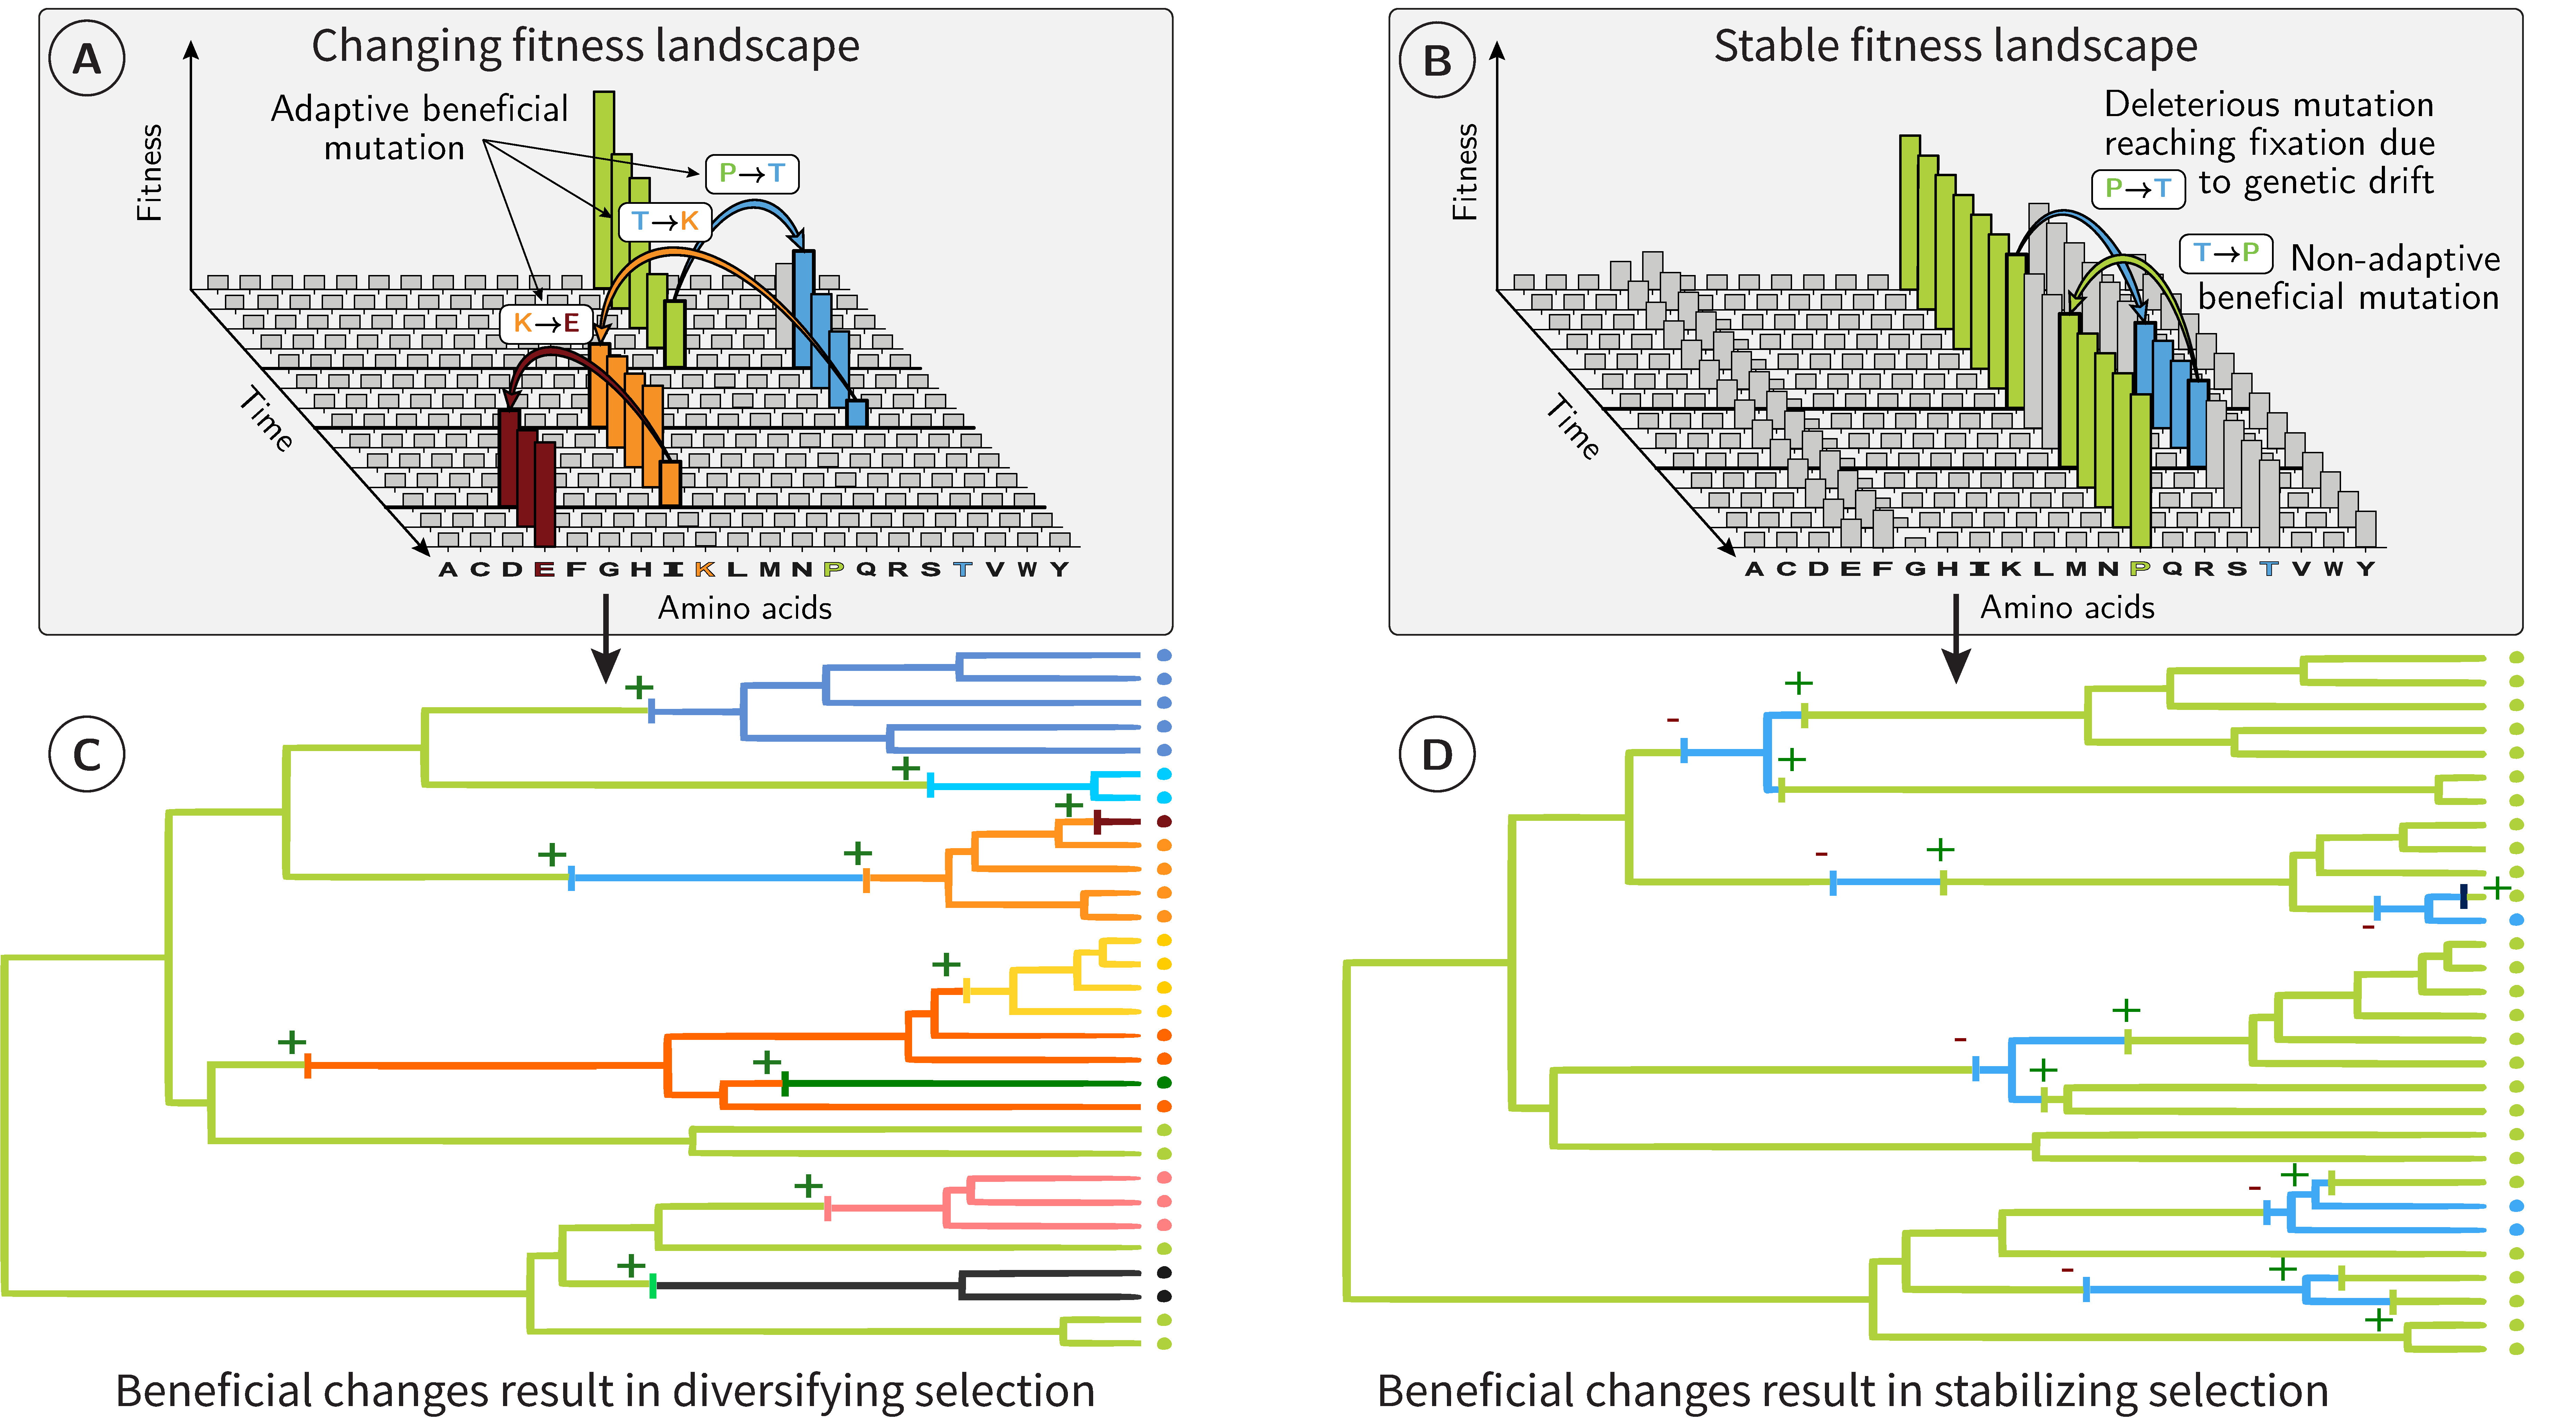
\includegraphics[width=\textwidth, page=1] {artworks/figure.fitness-landscape}
        \caption{
            Panel A and B: at a given site inside a protein-coding DNA sequence, the different amino acids (x-axis) have different fitnesses (y-axis).
            Under a fluctuating fitness landscape (panel A), these fitnesses are changing with time.
            The protein sequence is always lagging behind the moving target defined by the amino acid fitnesses, and since substitutions are accepted preferentially if they are in the direction of this target, substitutions are on average adaptive.
            At the phylogenetic scale (panel C), this phenomena promotes phenotype diversification across species.
            Under a stable fitness landscape (panel B), all the mutations reaching fixation are either slightly deleterious and reaching fixation due to drift, or are beneficial back-mutations restoring a more optimal amino acid.
            Scarce beneficial back-mutations are likely to reach fixation and a bulk of deleterious mutations are eventually reaching fixation due to their sheer mass.
            Across the genome, this process generate a balance at which genomes are constantly both damaged and repaired at different loci.
            At the phylogenetic scale (panel D), this phenomena promotes promotes phenotype stability and preserves well established biological systems.
        }
        \label{fig:fitness-landscape}
    \end{figure*}

    \begin{figure*}[!ht]
        \centering
        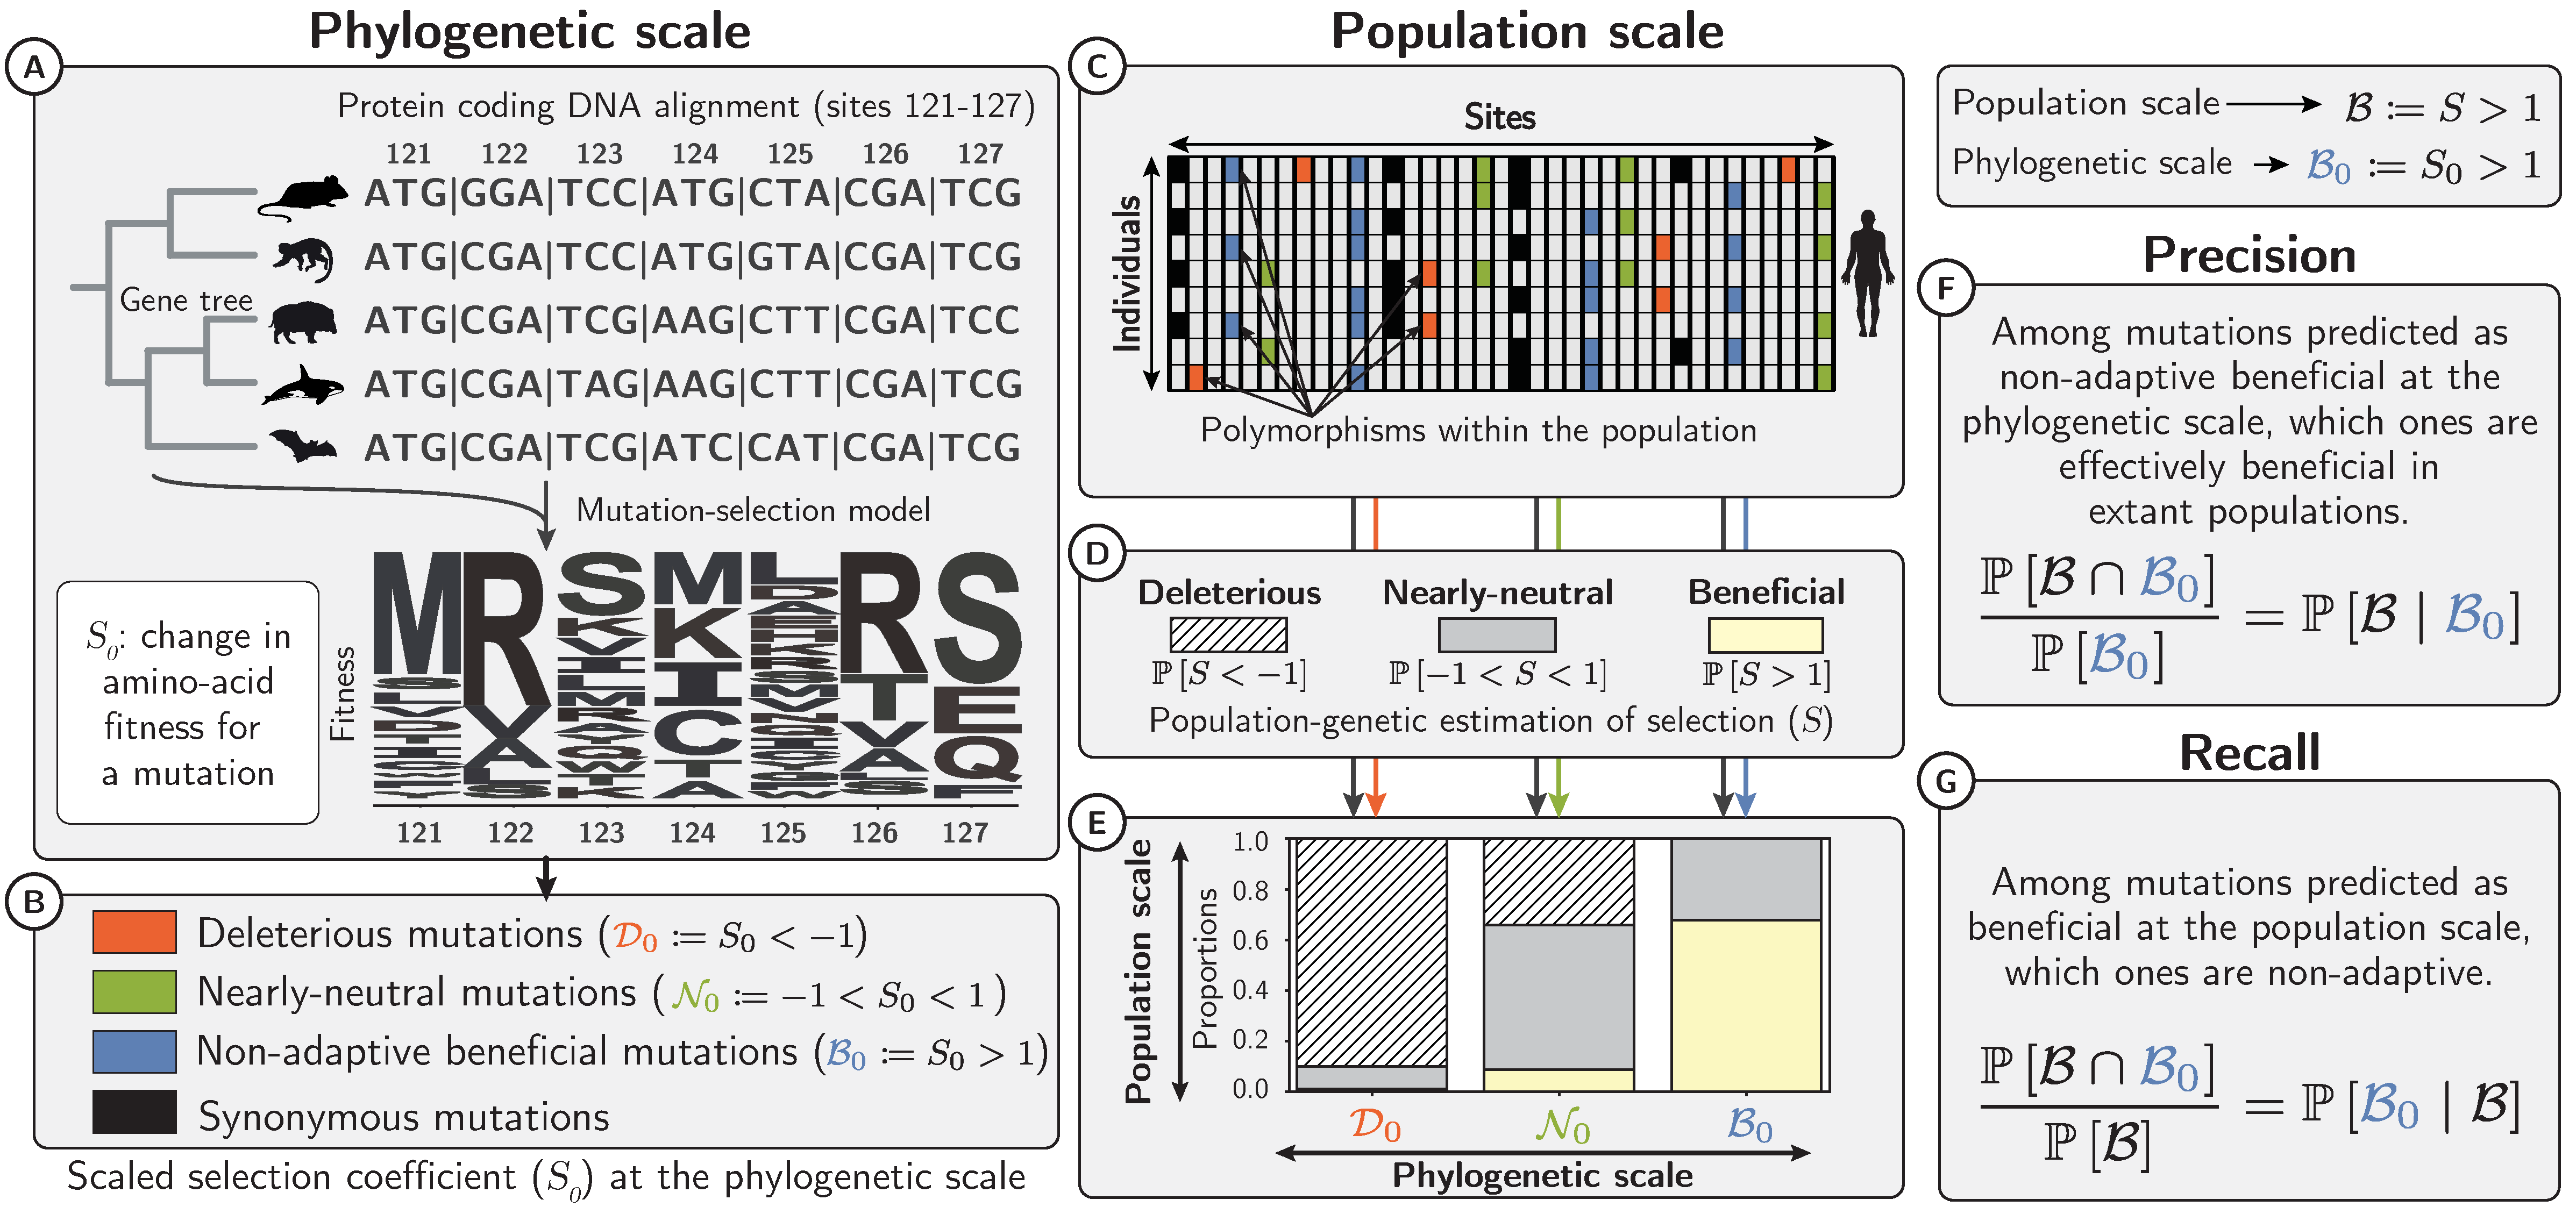
\includegraphics[width=\textwidth, page=1] {artworks/figure.method.proba}
        \caption{
            Integrating datasets at different scales.
            At the phylogenetic level (panel A), the amino acid Wrightian fitness for each site is estimated from protein-coding DNA alignments using mutation-selection codon models.
            Mutation-selection models assume a stable fitness landscape, taking into account only non-adaptive evolution.
            A mutation with a $\Sphy > 1$ would be driving the current site toward are fitter amino-acid, and such mutation are considered a beneficial back-mutation repairing existing functions (panel B).
            At the population scale (panel C), each single nucleotide polymorphism (SNP) segregating in the population can be classified as a beneficial back-mutation (in red) or not.
            The number of derived allele allow to estimate the probability of beneficial mutations at the population scale, for all SNPs or among back-mutations (panel D).
            The probability of back-mutation is obtained as their fraction among all possible mutations from the ancestral genome sequence (panel E).
            Altogether, we can estimate the probability of back-mutations among all beneficial ones, using Bayes' theorem (panel F).
        }
        \label{fig:method}
    \end{figure*}

    \subsection*{Back-mutations in the terminal lineages}
    We first probed for empirical evidence of beneficial back-mutation in the terminal lineages, which should be effectively beneficial.
    We thus reconstructed the substitutions occurring along the terminal branches of the phylogenetic tree.
    For each substitution, we estimated its scaled selection coefficient ($\Sphy$) based on the stable fitness landscape of amino-acids estimated at the scale of the mammals' phylogeny (fig.~\ref{fig:method}A).
    We showed that among all the substitutions in the terminal lineages, between 10 and 13\% had $\Sphy > 1$ (table~S1) and between 25 and 30\% had $\Sphy > 0$ (table~S2).
    Substitutions with $\Sphy > 1$ have been beneficial since the ratio of non-synonymous over synonymous divergence, called $\dnds$, was estimated to be between 1.15 and 1.68 in the different lineages (table~S1).
    This meant that beneficial back-mutations with $\Sphy > 1$ reach fixation more frequently than synonymous mutations, which are supposed to be neutral, thus are effectively beneficial.
    This also means that the ratio $\dnds$ usually used to detect adaptation while relying on substitutions between close species~\cite{mcdonald_adaptative_1991, galtier_adaptive_2016} or at the phylogenetic scale~\cite{goldman_codonbased_1994, yang_codonsubstitution_2002} is overinflated due to beneficial back-mutations.
    Then, $\dnds$ computed exclusively on non-synonymous sites with a $\Sphy < 0$ only represent the rate of evolution discarding beneficial back-mutations by construction.
    Thus, if we divide the $\dnds$ estimated on all substitutions by the one estimated only on substitutions predicted to be deleterious, we directly get the proportion of the rate of evolution which is contributed by beneficial back-mutations (see methods).
    This way, we estimated that between 22\% and 27\% of $\dnds$ is inflated because of beneficial back-mutations (table~S2).

    \subsection*{Back-mutations in the populations}
    Given that beneficial back-mutations are effectively selected for, we then ask which proportion of new mutations are beneficial back-mutations and are also beneficial at the population scale (fig.~\ref{fig:method}C-E).
    For each population with available polymorphism data, we first reconstructed the ancestral sequence (instead of the reference sequence) at the base of the population genealogy.
    From this reference sequence, we computed the scaled selection coefficient ($\Sphy$) for each possible non-synonymous mutations.
    We thus obtained the distribution of fitness effects (DFE) of new mutations from the ancestral sequence in \textit{Homo sapiens} (fig.~\ref{fig:homo-afr-results}A), under the assumption of the stable fitness landscape.
    Because $\Sphy$ is based on estimation of fitnesses at the mammalian scale, mutations with $\Sphy>1$ are considered beneficial back-mutations.
    Beneficial back-mutations only represents ~1.5\% of all possible new mutations (red in fig.~\ref{fig:homo-afr-results}A, table~S3).
    However, when focusing on the mutations that are observed in populations, namely single nucleotide polymorphism (SNP), beneficial back-mutations represents ~8.5\% of all observed mutations (red in fig.~\ref{fig:homo-afr-results}B, table~S3).

    Additionally, in populations, the frequencies at which SNPs are segregating is informative of their selective effect, e.g. deleterious SNPs are segregating at lower frequencies because they are purified.
    As such, methods have been developed to estimate the distribution of fitness effect (DFE) at the population scale by gathering information across many SNPs~\cite{eyre-walker_distribution_2006a, eyre-walker_estimating_2009a, galtier_adaptive_2016, tataru_inference_2017}.
    These methods offer a unique opportunity to compare the DFE at the population scale ($\Spop$) and at the phylogenetic scale ($\Sphy$).
    In order to estimate the DFE at the population level and gather robust statistical estimates, we grouped SNPs observed at the population level (e.g.~in humans of African descent in fig.~\ref{fig:homo-afr-results}) in 5 classes of predicted selection coefficient: severely deleterious with $\divStrongDel$, deleterious with $\divDel$, weakly deleterious with $\divWeakDel$, weakly beneficial with $\divWeakAdv$ and beneficial with $\divAdv$ (fig.~\ref{fig:homo-afr-results}B).
    In each of theses classes, the number of derived alleles in the population for each SNPs is used to generate a site-frequency spectrum (SFS) (fig.~\ref{fig:homo-afr-results}C).
    Compared to synonymous mutations which are supposedly neutral (black line in fig.~\ref{fig:homo-afr-results}C), mutations predicted to be deleterious (blue and green lines in fig.~\ref{fig:homo-afr-results}C) were, as expected, underrepresented at high frequencies in the population, a signature of ongoing purifying selection.
    However, these observations remain qualitative.

    To obtain a quantitative estimate of the distribution of selection coefficient for each category of SNPs, we used the model polyDFE~\cite{tataru_inference_2017, tataru_polydfe_2020}.
    This model uses the count of derived alleles for each frequency class of the SFS to infer the distribution of fitness effects (DFE) of the region under study.
    The model uses the number of sites ($L$) for each category (fig.~\ref{fig:homo-afr-results}A, see Material and Methods), the counts of synonymous derived allele as a neutral model, which allow to control for demographic effects, and polarization errors when inferring the ancestral state.
    We could estimate the proportion of beneficial mutations ($\PpolyAdv$), nearly-neutral mutations ($\PpolyNeutral$) and deleterious mutations ($\PpolyDel$) for each class of selection previously defined (fig.~\ref{fig:homo-afr-results}D).
    We found that SNPs predicted to be deleterious based on the selection coefficient $\Sphy$ estimated across the phylogeny of mammals were effectively purged at the population scale.
    Purifying selection is therefore largely predictable and amino acids with low fitness across mammals are effectively purged away in each population.
    Then, SNPs predicted to be beneficial based on the selection coefficient $\Sphy$ estimated at the scale of the phylogeny of mammals are indeed beneficial for individuals currently bearing them.
    These results confirmed that selection towards amino acids that are restoring existing function is ongoing in these populations.
    Between these two extreme cases, SNPs predicted to be weakly selected (cyan and orange in fig.~\ref{fig:homo-afr-results}) were effectively composed of neutral, beneficial and deleterious mutations.

    We replicated our experiment across 28 populations of different mammal species (fig.~\ref{fig:heatmap}) and found that SNPs predicted to be deleterious were indeed purged at the population scale (blue and green rows in fig.~\ref{fig:heatmap}A).
    However, SNPs predicted to be weakly beneficial ($\divWeakAdv$) were composed of a mix of neutral and selected mutations with varying proportions across the different populations (orange row in fig.~\ref{fig:heatmap}B).
    Finally, SNPs predicted to be beneficial back-mutations ($\divAdv$) were found to be beneficial with varying proportions across populations (red row in fig.~\ref{fig:heatmap}C).
    The variable proportions found between populations can be explained by the effective number of individuals in the population ($\Ne$), which is well-known to be a major driver of selection efficacy.
    Since $\Ne$ is not directly measurable, we used the Watterson $\theta_w$ as a proxy to order populations by their levels of synonymous diversity.
    Higher synonymous diversity is associated with a smaller proportion of nearly-neutral mutations (fig.~\ref{fig:diversity}A\&B).
    This result confirms the nearly-neutral theory and suggests that populations with higher diversity (e.g.~\textit{Bos} or \textit{Ovis}) are more likely to discriminate between beneficial and deleterious mutations (fig~S1-S9), while mutations in populations with low diversity (e.g.~\textit{Homo}) are effectively nearly-neutral.

    \subsection*{Proportion of back-mutations among all beneficial mutations}

    Finally, we propose an estimator for the probability of a beneficial mutation to be a beneficial back-mutation, i.e. $\mathbb{P} [ \Sphy > 1  \given  \Spop > 1]$ (fig.~\ref{fig:method}C-F).
    We obtained from the analyses above the following probabilities $\mathbb{P} [ \Sphy > 1 ]$, $\mathbb{P} [ \Spop > 1 ]$, $\mathbb{P} [ \Spop > 1  \given  \Sphy > 1]$.
    First, $\mathbb{P} [ \Sphy > 1 ]$ is the probability for a beneficial back-mutation ($\Sphy > 1$) from the ancestral sequence (red fill of histogram in fig~\ref{fig:homo-afr-results}A and table~S3).
    Second, $\mathbb{P} [ \Spop > 1 ]$ is the probability of mutation to be beneficial at the level of the population ($\Spop > 1$), estimated from all available SNPs (black fill in fig~\ref{fig:diversity}A and table~S3).
    Finally, $\mathbb{P} [ \Spop > 1  \given  \Sphy > 1]$ is the probability for a back-mutation ($\Sphy > 1$) to be effectively beneficial at the level of the population ($\Spop > 1$), when we restricted our analysis on SNPs that are already predicted to be beneficial back-mutations (black fill for the category $\Sphy > 1$ in fig~\ref{fig:homo-afr-results}D and table~S3).
    Combining these probabilities using Bayes theorem, we now obtain the probability for a beneficial mutation to be a back-mutation $\mathbb{P} [ \Sphy > 1  \given  \Spop > 1]$ (see Material and Methods).
    We estimated $\mathbb{P} [ \Sphy > 1  \given  \Spop > 1]$ across all populations sampled and obtained a proportion that varies between 10 and 26\% (table~S3).

    The proportion of back-mutations among all beneficial one did not show a clear relationship with the synonymous diversity within a population (Watterson $\theta_w$) (fig.~\ref{fig:diversity}C).
    Indeed, the relationship between $\Ne$ and the proportion of beneficial back-mutations is not trivial and should highly depend on time scales~\cite{charlesworth_other_2007}.
    A population that experienced a high $\Ne$ along its evolutionary time should be closer to the optimal state under a stable fitness landscape because of the higher efficacy of selection.
    This should decrease the probability of beneficial back-mutations.
    On the other hand, a high $\Ne$ over a short evolutionary time will induce more extreme fitness effects and a larger proportion of mutations will be beneficial (otherwise effectively neutral), thus increasing the proportion of beneficial back-mutations.
    Overall, the proportion of beneficial back-mutations is expected to be more dependent on effective population size contraction or expansion rather than on the short term effective population size captured by the synonymous diversity~\cite{charlesworth_other_2007}.

    \begin{figure*}[!ht]
        \centering
        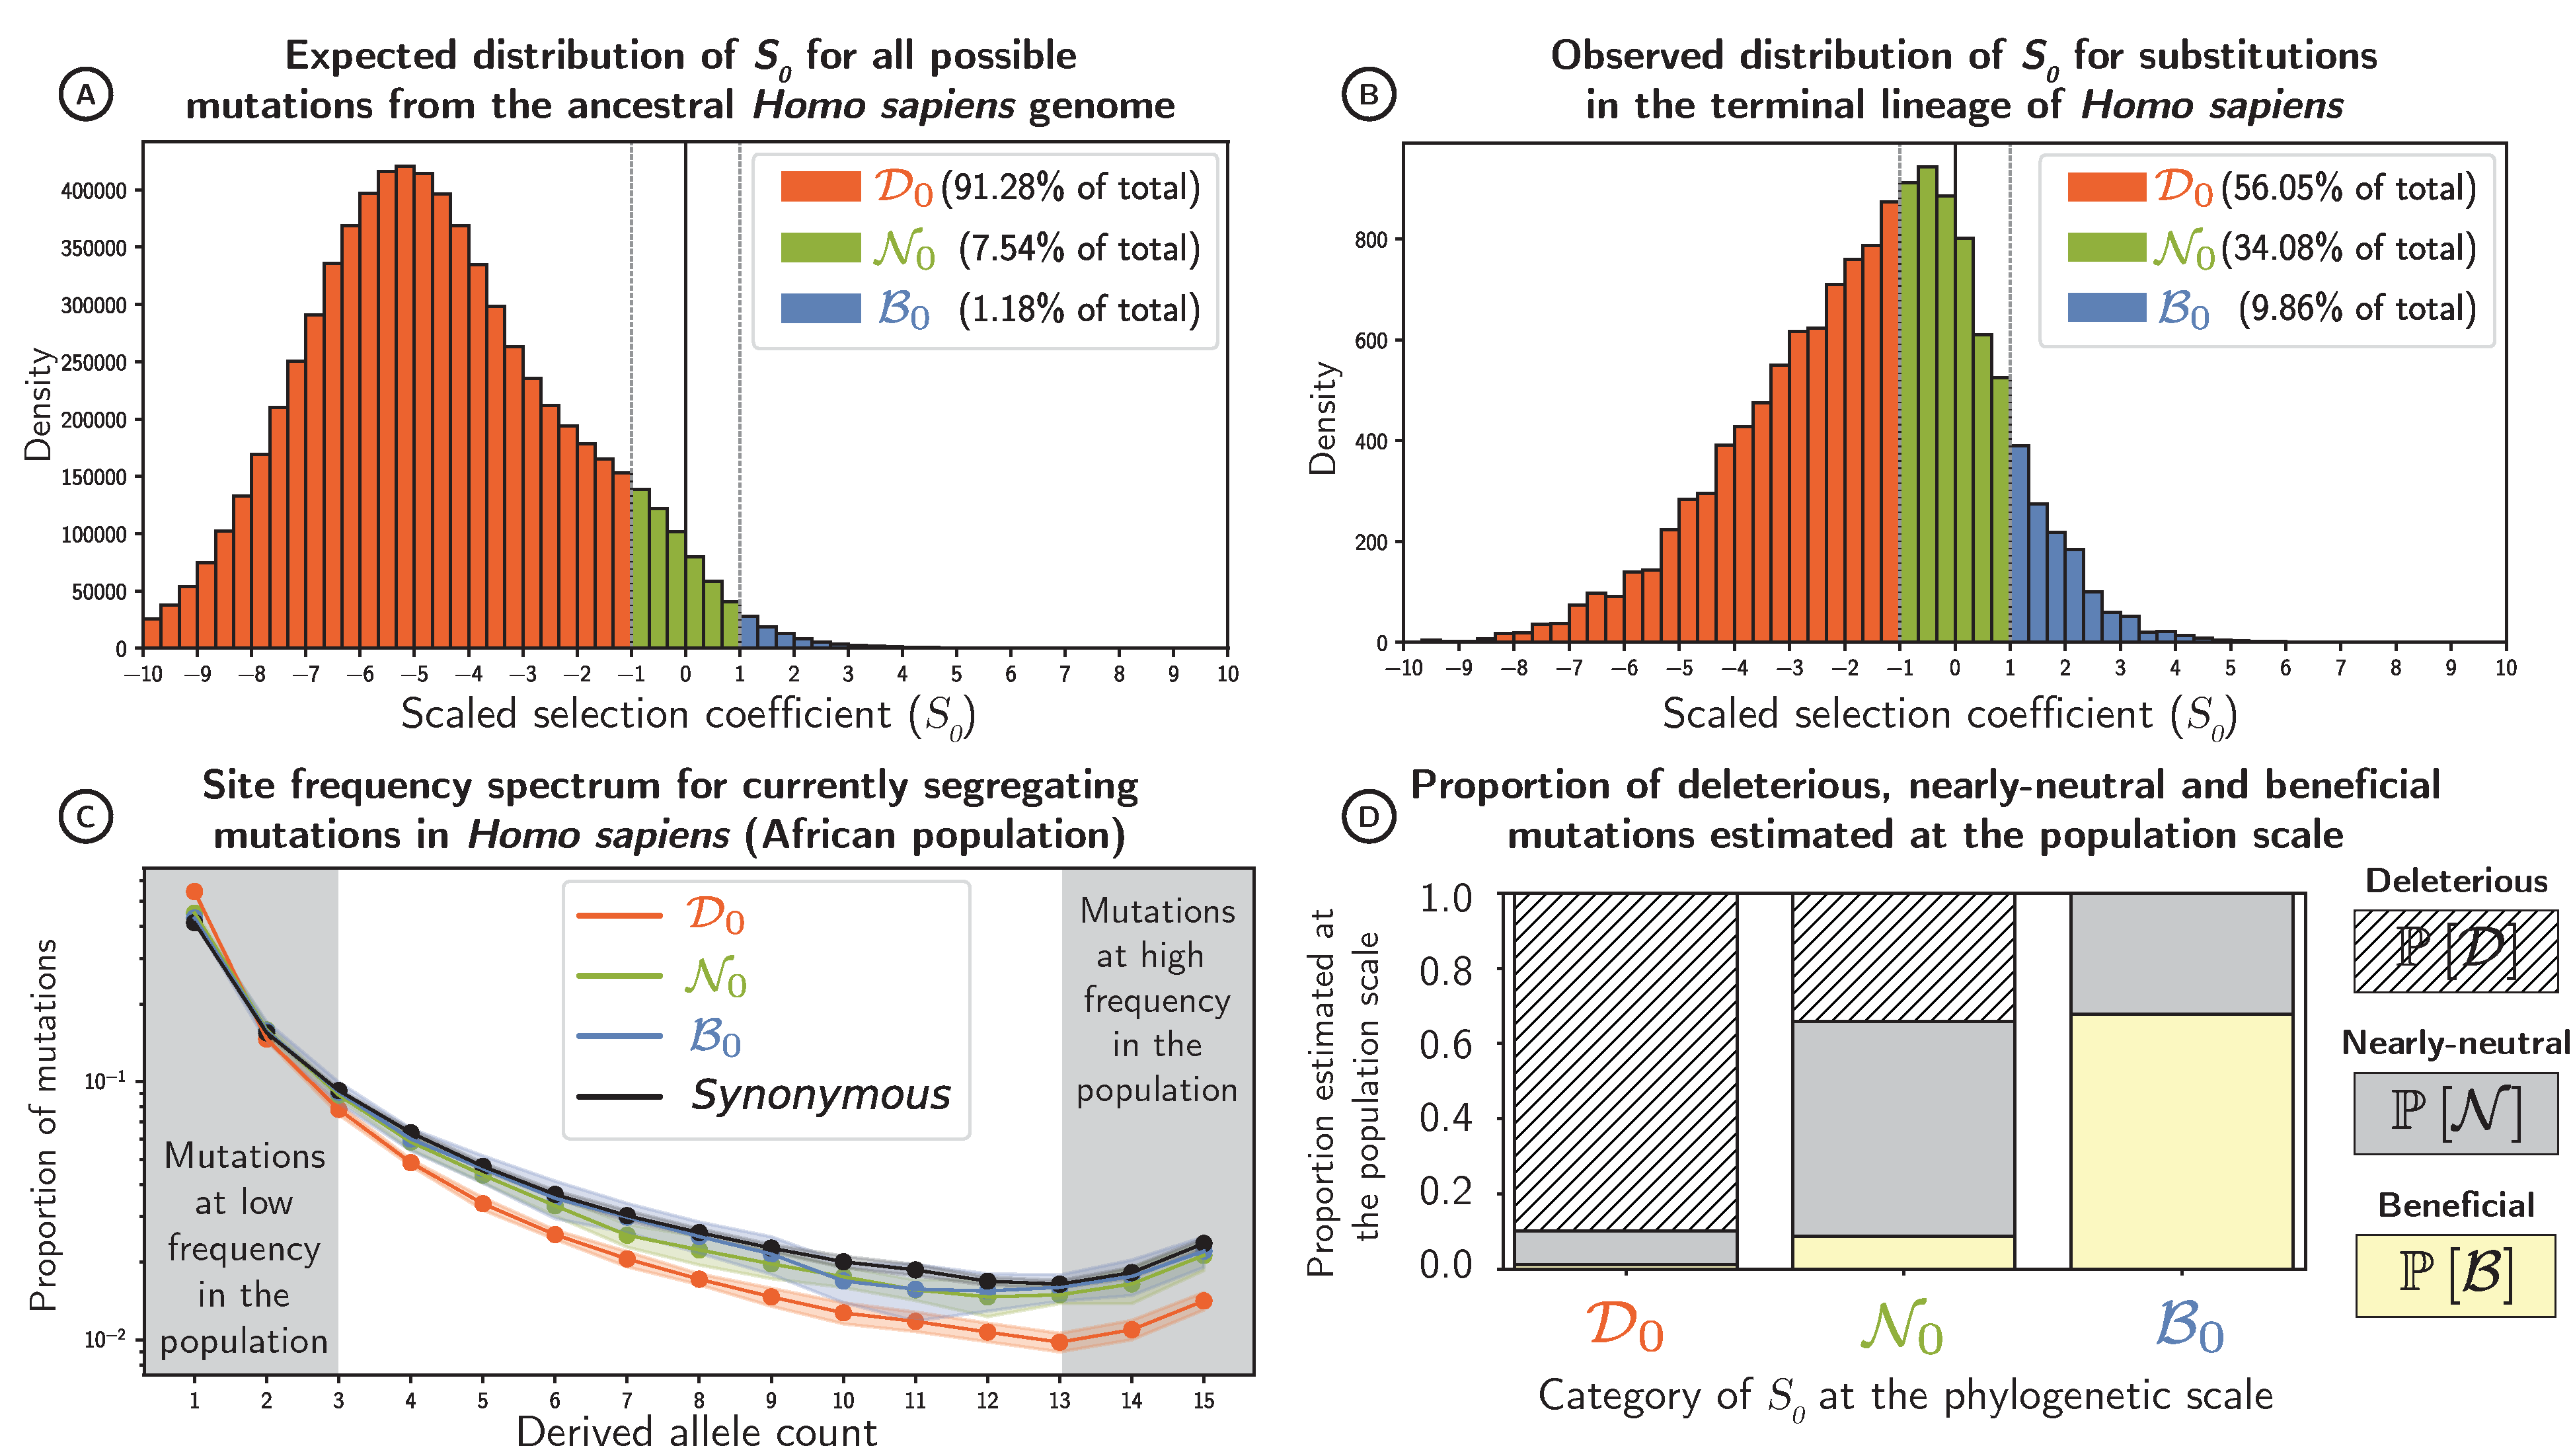
\includegraphics[width=\textwidth, page=1] {artworks/figure.homo-afr-results}
        \caption{
            Panel A: Distribution of fitness effects ($\Sphy$), predicted for all possible mutations away from the ancestral human genome.
            Mutations are divided into 5 classes of selection: severely deleterious (blue), deleterious (green), weakly deleterious (light green), weakly beneficial (yellow) and beneficial (red, supposedly beneficial back-mutations).
            Panel B. Distribution of fitness effects ($\Sphy$) for all observed SNPs in a sample of 8 individuals (out of 512 in the original dataset) of African descent.
            If they are less mutations observed than expected, this class is thus undergoing purifying selection.
            Panel B: The site-frequency spectrum (SFS) represents the proportion of mutations (y-axis) with a given number of derived alleles in the population (x-axis).
            SFS are drawn for a random sample of 16 alleles (mean in solid line and standard deviation in filled color) for each class of selection and for synonymous mutations which are supposedly neutral (black).
            At high frequencies, supposedly severally deleterious mutations are underrepresented.
            Panel D. For each class of selection (and for the set of all non-synonymous mutations), information from the SFS and the distribution of fitness effects are combined at the population scale to estimate the proportion of beneficial mutations $\PpolyAdv$, of nearly-neutral mutations $\PpolyNeutral$ and of deleterious mutations $\PpolyDel$.
        }
        \label{fig:homo-afr-results}
    \end{figure*}

    \begin{figure*}[!ht]
        \centering
        \includegraphics[width=\textwidth, page=1] {artworks/figure.heatmap}
        \caption{
            Reproducibility of results shown in figure~\ref{fig:homo-afr-results} in 28 populations across 6 genera.
            For each class of selection at the phylogenetic scale ($\Sphyclass \in \{ \divStrongDel, \divDel,  \divWeakDel,  \divWeakAdv, \divAdv \}$, in rows), site-frequency spectra and total number of sites are combined at the population scale to estimate the proportion of beneficial mutations ($\PpolyAdv$) in the top panel, of nearly-neutral mutations ($\PpolyNeutral$) in the middle panel and of deleterious mutations ($\PpolyDel$) in the bottom panel.
        }.
        \label{fig:heatmap}
    \end{figure*}

    \begin{figure*}[!ht]
        \centering
        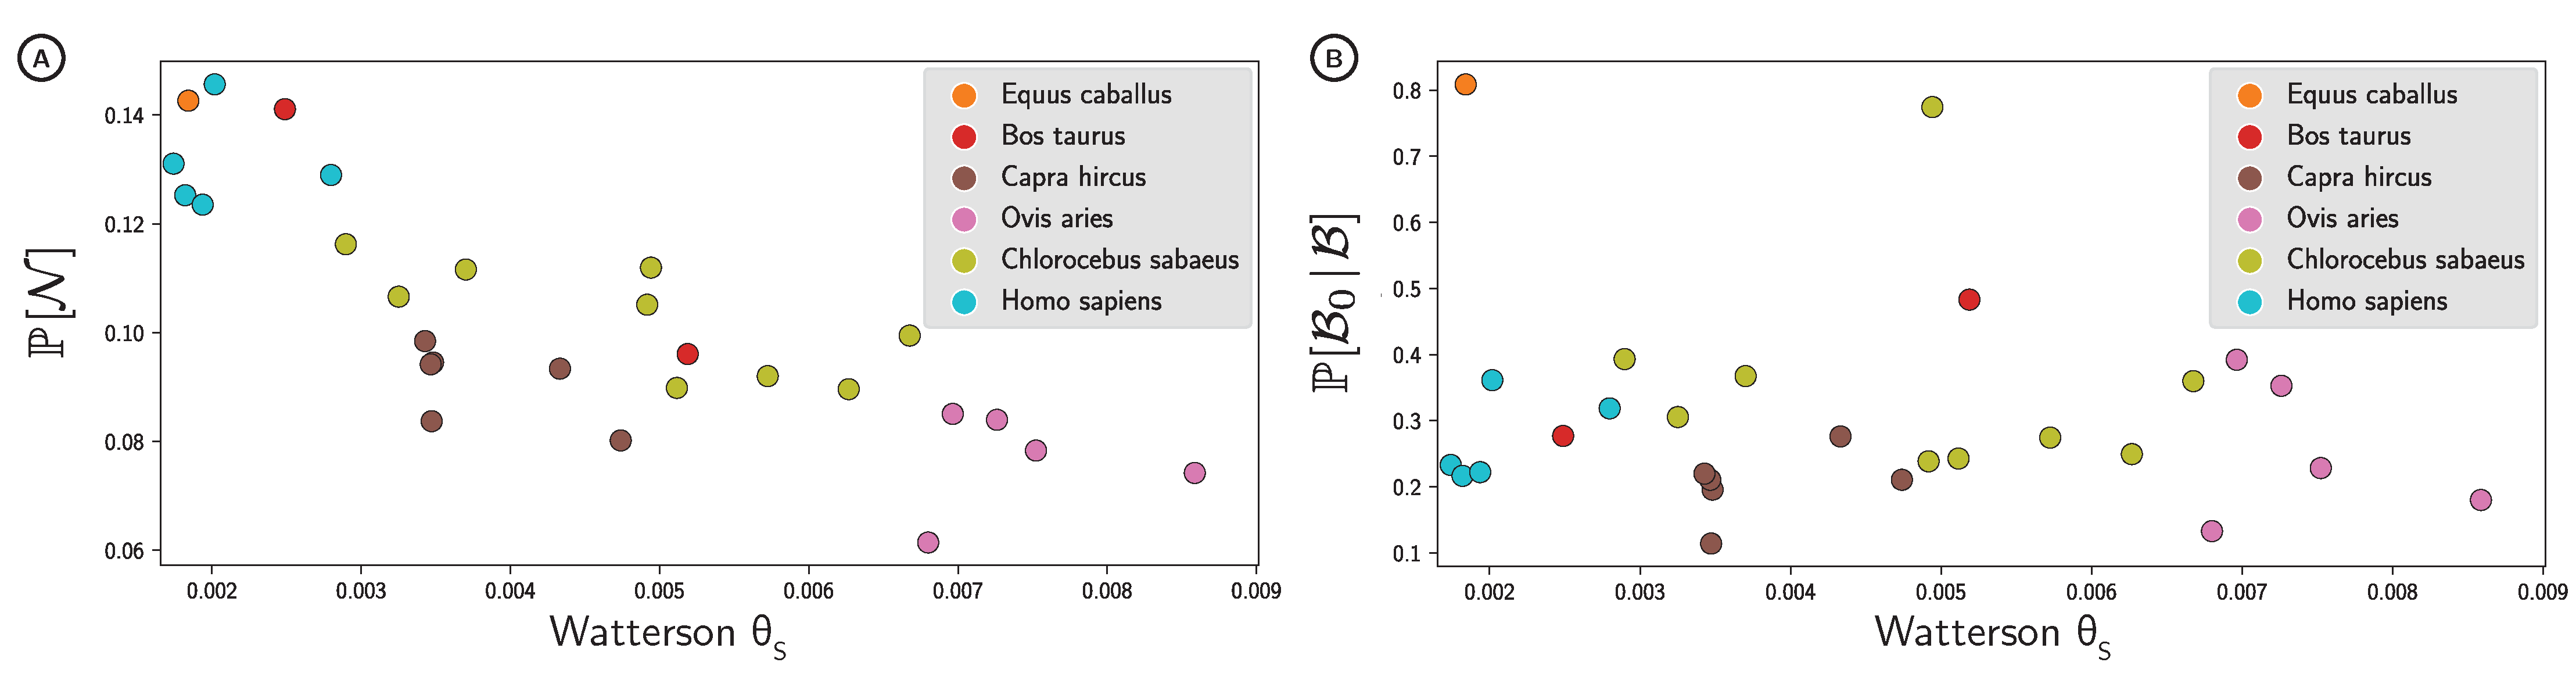
\includegraphics[width=\textwidth, page=1] {artworks/figure.diversity}
        \caption{
            Panel A. For each population, the proportion of beneficial ($\PpolyAdv$), nearly-neutral ($\PpolyNeutral$) and of deleterious ($\PpolyDel$) mutations estimated at the population scale using all SNPs available.
            Population are sorted for increased synonymous diversity.
            Panel B. Proportion of nearly-neutral mutations ($\mathbb{P} [ -1 < \Spop < 1]$ in y-axis), shown as a function of the synonymous diversity (Watterson $\theta_w$ in x-axis).
            Panel C. Proportion of beneficial back-mutations among all beneficial mutations ($\mathbb{P} [ \Sphy > 1  \given  \Spop > 1]$ in y-axis), shown as a function of the synonymous diversity (Watterson $\theta_w$ in x-axis).
        }
        \label{fig:diversity}
    \end{figure*}

    \subsection*{a bridge between phylogenetic and population-genetics}
    In this study, we first estimated selective effects of mutations inside protein coding sequence, under a model assuming no adaptation at the phylogenetic scale.
    We then estimated the proportion of beneficial mutations that are not adaptive innovations, and subsequently estimated their proportion among all beneficial mutations at the population scale.
    Our work confirms that deleterious substitutions have accumulated in mammals and are currently being eliminated, resulting in up to 25\% of beneficial mutations that are not adaptive innovations, but instead are repairing previous deleterious changes.

    From a theoretical evolution perspective, we have found that we can use phylogenetic signals and mutation-selection codon models to predict the selection coefficient of a mutation ($\Sphy$).
    However, we so far assumed no changes in effective population size along the phylogeny while it has been established that population size changes have a major effect on selection dynamics~\cite{lanfear_population_2014, jones_shifting_2017, platt_protein_2018}.
    Mutation-selection models with changes in effective population sizes along the phylogeny have been developed~\cite{latrille_inferring_2021a}, but are, for the moment, too computational intensive to be performed genome-wide.
    Hybrid mutation-selection and $\omega$-based codon models could provide a way forward to in integrate site-specific selection and branch-specific drift~\cite{brevet_reconstructing_2021a}.
    As for the estimate of selection, SIFT scores based on amino acid alignments across species have also been found to be informative of the selection pressure exerted at the population scale~\cite{chen_hunting_2021}.
    Our study indeed showed that sites with a higher SIFT score at the phylogenetic scale are more beneficial in the different populations (supp.\ mat\  section SIFT scores).
    In practice, SIFT scores are more coarse grained, with for example a bulk of mutations with a score of 1.0 (the highest), and does not provide a boundary between beneficial and deleterious mutations, nor are they based on population-genetic formalism.

    Biologically, another mechanism which generate non-adaptive beneficial mutations is compensatory mutations, which are repairing damage caused by deleterious mutations at another loci in the genome and generating a widespread signal of non-adaptative evolution~\cite{hartl_compensatory_1996, pollock_strong_2014, starr_epistasis_2016}.
    In our study we focused on mutations toward a more optimal amino-acid at a given site, not accounting for compensatory mutations since we assumed a model of fitness landscape without epistasis.
    As shown in other studies, these models without epistasis provide a reasonable estimate of average fitness profiles~\cite{youssef_consequences_2020}.
    But most importantly, we argue that our estimation of the amount of beneficial back-mutations is an underestimation, and that accounting for compensatory mutations by means of epistasis would mechanically increase our estimate.
    Indeed, a fluctuating fitness landscape due to an external forces (i.e. changes in environment) results in an acceleration of the rate of evolution~\cite{ rodrigue_detecting_2017, rodrigue_bayesian_2021}, which generates epistatic mutations that are immediately beneficial~\cite{gong_epistatically_2014}.
    In contrast, pervasive epistasis generates the opposite pattern, an entrenchment~\cite{goldstein_evolutionary_2004, goldstein_nonadaptive_2015} resulting in a slowing down of the rate evolution~\cite{rodrigue_detecting_2017, patel_epistasis_2022} or a standstill~\cite{youssef_evolution_2022}.
    In other words, under pervasive epistasis, finding empirical evidence for beneficial back-mutations is harder since restoring mutations become less and less likely to occur over time~\cite{goldstein_nonadaptive_2015, goldstein_sequence_2017, park_epistatic_2022}.
    Our study thus shows that beneficial back-mutations should not be overlooked, and we argue that both beneficial back-mutations and compensatory mutations play an important role in preventing our genome from collapsing under a mutation load.

    For the estimates of selection at the population scale ($\Spop$), there is no consensus on the expected shape of the DFE~\cite{welch_divergence_2008, bataillon_effects_2014}, although it has been found to be reliably constant between species~\cite{castellano_comparison_2019}.
    We used a model that allowed the inference of a full DFE by modelling the negative side of the DFE as a gamma distribution, and the positive side as an exponential distribution.
    However, when we aggregate SNPs that are expected to be strongly deleterious or strongly beneficial, the model struggles to fit their DFE to a gamma or an exponential distribution.
    As a result, while the proportions of deleterious/weakly-selected/beneficial mutations stays reliable, the mean values for selection coefficients ($\Spop$) estimated by polyDFE become biologically absurd ($\Spop \ll -10^3$).
    Such effect is not found for neutral SNPs and a method to accurately estimate the mean value of selection coefficients from SFS without assuming any shape for the DFE remains yet to be developed.
    Aside from methodological limitations, the mammalian case study might also not be representative of other clades.
    Indeed, mammals have relatively small long term population sizes, which allow large amounts of deleterious mutations to be fixed, and thus, there are a lot of opportunities for beneficial back-mutations to arise.
    It would thus be of great interest to reproduce our experiment with other clades, such as \textit{Drosophila} or birds which tend to have higher effective population size.
    It would also be interesting to have access to more shallow but wider phylogenies to increase the resolution of our predictions.

    From a structural biology perspective, we have found that proteins are not optimal for their fitness, which has been proved for their kinetics and thermodynamics~\cite{hartl_compensatory_1996, taverna_why_2002, goldstein_evolution_2011}.
    Philosophically, our distinction between beneficial back-mutations and adaptation can appear to be far-fetched, and one can argue that beneficial back-mutations is adaptation to its own deteriorating genome.
    However, there is a difference between adapting to a mutation, for instance by the mean of a compensatory mutation elsewhere, and cancelling the mutation, by the mean of a substitution on the misfit amino-acid.
    The first still implies changes in the genetic sequence and thus genetic diversification, while the second reduces the diversity.
    We also argue that this distinction is important when we seek to detect adaptation, and is actually not an encumbrance but rather a strength.
    Precisely, mutation-selection models are genuinely taking into account the tug-of-war between scarce beneficial mutations likely to reach fixation and a bulk of deleterious mutations eventually reaching fixation due to their sheer mass.
    These models can thus be used as a null model to predict the expected rate of evolution of proteins~\cite{spielman_relationship_2015, dosreis_how_2015} under a stable fitness landscape.
    A departure from this model indicates that proteins are evolving under a changing fitness landscape~\cite{cvijovic_fate_2015, rodrigue_detecting_2017, tamuri_mutationselection_2021} and is a signal of pervasive adaptive evolution~\cite{rodrigue_bayesian_2021} or of pervasive epistasis~\cite{rodrigue_detecting_2017}.
    As such, a stable fitness landscape as a null model is thus statistically more powerful to detect adaptation than assuming that the null model is neutral evolution.
    Taken together, mutation-selection models are a mandatory tool in evolutionary biology to detect and quantify adaptation at the phylogenetic scale, while acknowledging beneficial back-mutations.

    In conclusion, we showed that by integrating genome-wide datasets at the phylogeny and the population scale, it is possible to estimate the proportion of beneficial mutations repairing existing functions instead of generating adaptive innovations.
    We argue that our approach is general and our methodology can be readily applied to different estimations of fitness landscape at the phylogenetic scale, and different models and methods estimating distribution of fitness effects at the population scale.
    This study at the interface between phylogenetic and population-genetics thus provide a step toward an integration of different scales necessary to decipher the combined effects of mutation, selection and drift on genome evolution.


    \section*{Acknowledgments}
    \label{sec:acknowledgment}
    We gratefully acknowledge the help of Mélodie Bastian, Nicolas Lartillot, Laurent Duret and Diego A. Hartasánchez Frenk for their advices and reviews concerning this manuscript.
    This work was performed using the computing facilities of the CC LBBE/PRABI\@.
    This study makes use of data generated by the NextGen Consortium.
    The European Union’s Seventh Framework Programme (FP7/2010-2014) provided funding for the project under grant agreement no 244356 - “NextGen”.
    \textbf{Funding:}
    Université de Lausanne; Agence Nationale de la Recherche, Grant ANR-19-CE12-0019 / HotRec.
    \textbf{Author contributions:}
    Original idea: T.L.\ and J.J.;
    Model conception: T.L., J.J.\ and N.S.;
    Code: T.L.;
    Data analyses: T.L.\ and J.J.;
    Interpretation: T.L., J.J.\ and N.S.;
    First draft: T.L.\ and J.J.;
    Editing and revisions: T.L., J.J.\ and N.S.
    Project management and funding: N.S\@.
    \textbf{Competing interests:}
    The authors declare no conflicts of interest.
    \textbf{Data and materials availability:}
    Snakemake pipeline, analysis scripts and documentation are available at \href{https://github.com/ThibaultLatrille/SelCoeff}{github.com/ThibaultLatrille/SelCoeff}.


    \section{Material \& Methods}
    \label{sec:methods}

    \subsection{Phylogenetic dataset}

    Protein-coding DNA sequences alignments in placental mammals and their corresponding gene trees were extracted from the \href{https://www.orthomam.univ-montp2.fr}{OrthoMaM} database.
    It contained a total of $116$ mammalian reference sequences in v10c~\cite{ranwez_orthomam_2007, douzery_orthomam_2014, scornavacca_orthomam_2019}.
    Genes located on the X, Y chromosomes and the mitochondrial genome were discarded from the analysis, because the level of polymorphism, which is necessary in the population-based analyses, is expected to be different in these three genomic regions.
    Sequences of species for which we used population-level polymorphism (see below), as well as their sister species, were removed from the analysis to ensure independence between the data used in the phylogenetic and population scale.
    Altogether, we analyzed $14,509$ protein-coding DNA sequences for at most $87$ sequences of placental mammals.

    \subsection{Selection coefficient ($\Sphy$) in phylogeny-based method}
    \label{subsec:s-phylogeny-method}

    We analyzed the phylogenetic level data using mutation-selection models.
    These models assume that the protein-coding sequence are at mutation-selection balance under a fixed fitness landscape characterized by a fitness vector over the $20$ amino acid at each site~\cite{yang_mutationselection_2008, halpern_evolutionary_1998, rodrigue_mechanistic_2010}.
    Mathematically, the rate of non-synonymous substitution from codon $a$ to codon $b$ ($q_{a \mapsto b}^{(i)}$) at site $i$ of the sequence is equal to the rate of mutation of the underlying nucleotide change ($\mu_{a \mapsto b}$) multiplied by the scaled probability of fixation of the mutation ($\proba_{a \mapsto b}^{(i)}$).
    The probability of fixation depends on the difference of scaled fitness of the amino acid encoded by the mutated codon ($F_b^{(i)}$) and the amino acid encoded by the original codon ($F_a^{(i)}$) at site $i$~\cite{wright_evolution_1931a, fisher_genetical_1930a}.
    The rate of substitution from codon $a$ to $b$ at a site $i$ is thus:
    \begin{equation}
        \begin{dcases}
            q_{a \mapsto b}^{(i)} & = 0 \text{ if codons $a$ and $b$ are more than one mutation away,} \\
            q_{a \mapsto b}^{(i)} & = \mu_{a \mapsto b} \text{ if codons $a$ and $b$ are synonymous,} \\
            q_{a \mapsto b}^{(i)} & = \mu_{a \mapsto b} \dfrac{F_b^{(i)} - F_a^{(i)}}{1 - \e^{F_a^{(i)} - F_b^{(i)}}} \text{ if codons $a$ and $b$ are non-synonymous}.
        \end{dcases}
    \end{equation}
    Fitting the mutation-selection model on a sequence alignment leads to an estimation of the mutation rate matrix ($\UniDimArray{\mu}$) as well as the 20 amino acid fitness landscape ($\UniDimArray{F^{(i)}}$) at each site $i$.
    The selection coefficient for a mutation from codon $a$ to codon $b$ at site $i$ is defined :
    \begin{equation}
        \Sphy^{(i)} (a \mapsto b) = \Delta F^{(i)} = F^{(i)}_{b} - F^{(i)}_{a}.
    \end{equation}
    In the manuscript and the following material, the source ($a$) and target ($b$) codons as well as the site ($i$) are implicit and thus never explicitly written.
    We ran the Bayesian software \textit{BayesCode} (\url{https://github.com/ThibaultLatrille/bayescode}) on each protein-coding DNA alignment~\cite{rodrigue_bayesian_2021}.
    We ran a Markov chain Monte-Carlo (MCMC) analysis during $2000$ generations, with a burn-in period of $1000$ generations, to obtain posterior mean estimates of the amino acid fitness landscape ($\UniDimArray{F^{(i)}}$) at each site $i$\@.

    \subsection{Polymorphism dataset}
    \label{subsec:polymorphism-dataset}

    We retrieved the genetic variants representing the population level polymorphism from the following species and respective available datasets: \textit{Equus caballus} (EquCab2 assembly in the EVA study PRJEB9799~\cite{alabri_whole_2020}), \textit{Bos taurus} (UMD3.1 assembly in the NextGen project: \url{https://projects.ensembl.org/nextgen/}), \textit{Ovis aries} (Oar\_v3.1 assembly in the NextGen project: \url{https://projects.ensembl.org/nextgen/}), \textit{Capra Hircus} (CHIR1 assembly in the NextGen project: \url{https://projects.ensembl.org/nextgen/}, liftover to the ARS1 assembly), \textit{Chlorocebus sabaeus} (ChlSab1.1 assembly in the EVA project PRJEB22989~\cite{svardal_ancient_2017}), \textit{Homo sapiens} (GRCh38 assembly from the 1000-genome project~\cite{consortium_integrated_2012a, the1000genomesprojectconsortium_global_2015}).
    In total, we analyzed 28 populations across the 6 different species with polymorphism data.
    Genetic variants that were not found within a gene were not used in further analyses.
    We also did not analyzed insertions and deletions and focused only on Single Nucleotide Polymorphisms (SNPs) with a single mutant allele.
    Finally, stop codon mutants were also discarded.

    Each SNP (chromosome, position, strand) in the focal species was matched to its relative position (chromosome, position, strand) in the protein-coding DNA alignment by first converting the genomic positions to relative position in the coding sequence (CDS) using gene annotation files (GTF format) downloaded from Ensembl (\url{ensembl.org}).
    We then verified that the SNP downloaded from Ensembl were matching the reference in the CDS (FASTA format).
    Second, the relative position in the CDS was converted to position in the multiple sequence alignment (containing gaps) from OrthoMaM database~\cite{ranwez_orthomam_2007, douzery_orthomam_2014, scornavacca_orthomam_2019} by doing a global pairwise alignment, using the Biopython function pairwise2, between the CDS fasta and the sequence found in the alignment.
    This conversion from genomic position to position in the alignment is only possible if the assembly used for SNP calling is the same as the one used in the alignment, the GTF annotations and the FASTA sequences.
    SNPs were polarized using the $3$ closest outgroups found in the OrthoMam alignment with est-usfs v2.04~\cite{keightley_inferring_2018}.
    For populations containing more than $8$ individuals, the site-frequency spectrum (SFS) was subsampled down to $16$ chromosomes ($8$ diploid individuals) without replacement (hyper-geometric distribution) to alleviate the effect of different sampling depth in the 28 populations.
    We developped a Snakemake pipeline to integrate polymorphism and divergence data with custom scripts written in python 3.9.

    \subsection{Selection coefficient ($\Spop$) in population-based method}
    \label{subsec:s-polymorphism-method}
    The probability to sample an allele at a given frequency (before fixation or extinction) is informative of its scaled selection coefficient at the population scale ($\Spop$).
    Pooled across many sites, the SFS provides therefore information on the underlying $\Spop$ of mutations.
    However, estimating a single $\Spop$ for all sampled mutations is biologically unrealistic and a distribution of fitness effects of mutations (DFE) is usually assumed~\cite{eyre-walker_distribution_2006a, eyre-walker_estimating_2009a}.
    In this study, we used the software polyDFE~\cite{tataru_inference_2017, tataru_polydfe_2020}, which used a mixture of a $\Gamma$ and Exponential distributions to model the DFE of non-synonymous mutations, while synonymous mutations are considered neutral.
    The model estimates the parameters $\Spop_d$ , $b$, $p_b$ and $\Spop_b$ for non-synonymous mutations as:
    \begin{equation}
        \phi \left( \Spop; \Spop_d , b, p_b, \Spop_b \right) =
        \begin{dcases}
            \left( 1 - p_b \right) f_{\Gamma}(-\Spop; -\Spop_d, b) & \text{ if $\Spop \leq 0$,} \\
            p_b f_{e}(\Spop; \Spop_b) & \text{ if $\Spop > 0$,} \\
        \end{dcases}
    \end{equation}
    where $\Spop_d \leq -1 $ is the estimated mean of the DFE for $\Spop \leq 0$,
    $b \geq 0.4$ is the estimated shape of the $\Gamma$ distribution,
    $0 \leq p_b \leq 1$ is the estimated probability that $\Spop > 0$,
    $\Spop_b \geq 1$ is the estimated mean of the DFE for $\Spop > 0$,
    and $f_{\Gamma}(x; m, b)$ is the density of the $\Gamma$ distribution with mean m and shape b, while $f_{e}(x; m)$ is the density of the Exponential distribution with mean $m$.
    Once the DFE was fitted to the data, the proportion of beneficial ($\PpolyAdv$), nearly-neutral ($\PpolyNeutral$) and deleterious mutations ($\PpolyDel$) were given as:
    \begin{align}
        \PpolyAdv &= p_b \int_{1}^{+\infty} f_{e}(\Spop; \Spop_b) \der \Spop,  \label{eq:polyProbaAdv} \\
        \PpolyNeutral &= p_b \int_{0}^{1} f_{e}(\Spop; \Spop_b) \der \Spop + \left( 1 - p_b \right) \int_{0}^{1} f_{\Gamma}(\Spop; -\Spop_d, b) \der \Spop, \\
        \PpolyDel &= \left( 1 - p_b \right) \int_{1}^{+\infty} f_{\Gamma}(\Spop; -\Spop_d, b) \der \Spop. \label{eq:polyProbaDel}
    \end{align}

    PolyDFE required one SFS for non-synonymous mutatipons and one for synonymous mutations (neutral expectation), as well as the number of sites on which each SFS has been sampled.
    We performed the following four-step procedure to obtain the number of sites for each SFS.
    First, for each population with polymorphism data available, the polarized SNPs (ancestral and derived alleles) were used to reconstruct the ancestral DNA sequence, containing only substitutions and no segregating polymorphisms.
    If a SNP is still segregating in the population, the ancestral version of the SNP is used.
    However, if the derived allele is shared by all individuals in the population, the allele is considered fixed and the derived allele of the SNP is used as the ancestral.
    Second, from this reconstructed ancestral sequence, all possible mutations were computed, weighted by the mutation rate between nucleotide ($\mu$), which was estimated at the phylogenetic scale.
    Third, the total mutation rate for synonymous mutations, called $\mu_{\textrm{syn}}$, was estimated as the sum across the whole genome.
    Similarly, the total mutation rate for each class of selection, called  $\mu\left( \Sphyclass \right)$, was estimated as the sum across all non-synonymous mutations if their selection coefficient at the phylogenetic scale ($\Sphy$) was in the class $\Sphyclass$ (e.g. $\Sphyclass = \divAdv$).
    Fourth, the number of sites ($L \left( \Sphyclass \right)$) for each class of selection coefficient ($\Sphyclass$) was finally computed as the total number of sites across the genome ($L_{tot}$) weighted by the ratio of the aggregated mutations rates falling in the class ($\mu\left( \Sphyclass \right)$) over the total mutation rate for all possible mutations ($\mu_{tot}$) as:
    \begin{align}
        L \left( \Sphyclass \right) &= L_{tot} \frac{\mu\left( \Sphyclass \right)}{\mu_{tot}}, \\
        L_{\textrm{syn}} &= L_{tot} \frac{\mu_{\textrm{syn}}}{\mu_{tot}}.
    \end{align}

    Altogether, for each class of selection ($\Sphyclass$) of non-synonymous SNPs (or for all SNPs), we thus estimated the parameters of the DFE $\left( \Spop; \Spop_d , b, p_b, \Spop_b \right)$ using maximum likelihood with polyDFE from the number of sites and the SFS obtained by aggregating all the SNPs in the selection class.
    Once fitted to the data, the parameters of the DFE $\left( \Spop; \Spop_d , b, p_b, \Spop_b \right)$ are used to compute $\PpolyAdv$, $\PpolyNeutral$, $\PpolyDel$ using eq.~\ref{eq:polyProbaAdv}-\ref{eq:polyProbaDel}.

    From Bayes theorem, it is now possible to obtain the probability for a beneficial mutation to be a back-mutation .
    In other words, we seek to get the probability that a mutation is repairing the genome ($\divAdv$) given that it is beneficial ($\polyAdv$), as:
    \begin{equation}
        \proba \left[\divAdv \given \polyAdv\right] = \frac{\proba \left[\polyAdv \given \divAdv\right] \times \proba\left[\divAdv\right]}{\PpolyAdv},
        \label{eq:bayes}
    \end{equation}
    where $\PpolyAdv$ is computed from all SNPS, $\proba \left[\polyAdv \given \divAdv\right]$ is obtained from the set of SNPs in the class $\Sphyclass = \divAdv$, and $\proba\left[\divAdv\right]$ is the probability for a new mutation to be inside the class $\divAdv$, thus computed as:
    \begin{equation}
        \proba\left[\divAdv\right] = \frac{\mu\left( \Sphyclass = \divAdv \right)}{\mu_{tot}},
        \label{eq:proba-dfe-mutsel}
    \end{equation}

    \subsection*{Substitution mapping in the terminal branch}
    \label{subsec:substitution-mapping-in-the-terminal-branch}
    For each gene and for each population with polymorphism data available, the ancestral DNA sequence was reconstructed from ancestral and fixed polymorphism (see previous section).
    Then, using this ancestral DNA reference and the $3$ closest outgroups found in the OrthoMam alignment, we reconstructed the ancestral protein-coding DNA sequences for each node of the 4-leaves tree with the yang M5 codon model (gamma site rate variation) in FastML.v3.11~\cite{ashkenazy_fastml_2012}.
    All polarized codon substitutions are then obtained by comparing the ancestral protein-coding DNA sequences before the split to the sister species (closest outgroup) to the ancestral DNA reference for the population of interest (without segregating polymorphism).
    We considered \textit{Ceratotherium simum simum} as \textit{Equus caballus} sister species; \textit{Bison bison bison} as \textit{Bos taurus} sister species; \textit{Pantholops hodgsonii} as \textit{Ovis aries} sister species; \textit{Pantholops hodgsonii} as \textit{Capra Hircus} sister species; \textit{Macaca mulatta} as \textit{Chlorocebus sabaeus} sister species and finally we considered \textit{Pan troglodytes} as \textit{Homo sapiens} sister species.
    The selection coefficient ($\Sphy$) of each substitution is then obtained by comparing the difference in amino acid fitnesses for each polarized non-synonymous codon substitution, by referring to the site-specific fitness profile obtained in the phylogeny-based method (see~\ref{subsec:s-phylogeny-method}).
    Finally, the rate of non-synonymous over synonymous substitution for a given class of selection coefficient ($\Sphyclass$) is computed as:
    \begin{align}
        \dn \left( \Sphyclass \right) &= \dfrac{D\left( \Sphyclass \right)}{L \left( \Sphyclass \right)}, \\
        \ds &= \dfrac{D_{\textrm{syn}}}{L_{\textrm{syn}}},
    \end{align}
    where $D \left( \Sphyclass \right) $ is the number of non-synonymous substitutions in the class $\Sphyclass$, $D_{\textrm{syn}}$ is the number of synonymous substitutions across the genome, while $L \left( \Sphyclass \right)$ and $L_{\textrm{syn}}$ are the number of non-synonymous and synonymous sites as defined in the previous section.
    The fraction of non-adaptive beneficial substitutions $R(\dnds)$ was computed as the ratio between the difference in the numbers of beneficial substitutions ($\dnds$), which were due to beneficial back-mutations, and the estimated divergence when we removed beneficial back-mutations $\dn (\Sphy < 0) / \ds$, over $\dnds$.
    Of note, the quantities $R(\dn)$ and $R(\dnds)$ are equivalent due to simplification of the factor $\ds$:
    \begin{equation}
        R(\dnds) = \dfrac{\dnds - \dn(\Sphy < 0) / \ds}{\dnds} = \dfrac{\dn - \dn(\Sphy < 0)}{\dn} = R(\dn)
    \end{equation}

    \printbibliography
\end{document}
